\chapter{Création du modèle de détection de fraude : Étapes 4 et 5}
\label{chap:creation-modele}

Dans la suite de l'analyse, l'étude se concentre sur trois approches de modélisation couramment utilisées en détection de fraude :

\begin{itemize}
    \item Un \textbf{modèle de \textit{Scoring} en points} (interprétable et proche des pratiques actuarielles traditionnelles) ;
    \item Un \textbf{arbre de décision} (permettant de capturer des effets non linéaires et des interactions) ;
    \item Un \textbf{modèle de type Gradient Boosting} (plus performant en général grâce aux méthodes d'ensemble).
\end{itemize}

L'objectif est d'évaluer et de comparer leur \textbf{qualité de prédiction} à partir de métriques adaptées, tout en tenant compte des enjeux d'interprétabilité et d'implémentation opérationnelle.

Dans ce cadre, l'outil développé propose dans un premier temps de sélectionner un partitionnement de la base globale de manière à définir deux jeux de données :

\begin{itemize}
    \item Un jeu qui servira de base d'apprentissage ;
    \item Un jeu qui servira de base de test du modèle créé.
\end{itemize}

Le choix du partitionnement est laissé à l'utilisateur, avec une valeur par défaut de départ à 80/20 (ratio base d'apprentissage/base de test) correspondant aux proportions généralement utilisées lors de la mise en place de modèles sur ce type de volumétrie de données.

\begin{figure}[H]
    \centering
    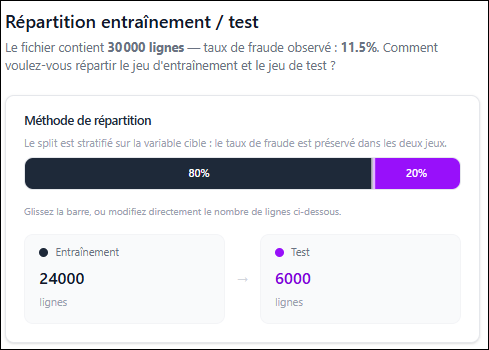
\includegraphics[width=0.7\textwidth]{images/chapitre5/partition.png}
    \caption{Choix du partitionnement de la base}
    \label{fig:partition}
\end{figure}

Pour notre exemple, une partition \textbf{80 / 20} est retenue : 80~\% des observations (24\,000 lignes) constituent le jeu d'apprentissage-validation, et les 20~\% restants (6\,000 lignes) forment le jeu de test final, mis de côté dès le départ et non utilisé pendant la phase de construction.

Ce partitionnement est \textbf{stratifié sur la variable cible}, ce qui signifie que le taux de fraude observé (11,5~\%) est préservé à l'identique dans les deux jeux. Cette précaution est essentielle sur des données déséquilibrées : un tirage purement aléatoire pourrait sur- ou sous-représenter les cas de fraude dans l'un des jeux, faussant l'apprentissage comme l'évaluation.

Sur la portion d'apprentissage-validation (80~\%), une \textbf{validation croisée à 5 plis} est appliquée pour la sélection des hyperparamètres. Le principe consiste à diviser ces données en cinq sous-ensembles : le modèle est entraîné à cinq reprises, chaque fois sur quatre plis et évalué sur le cinquième, de sorte que chaque observation serve tour à tour à l'entraînement et à la validation. Cette approche fournit une estimation plus robuste de la performance et limite le risque de sur-ajustement (\textit{overfitting}) au moment du choix des paramètres.

Enfin, le jeu de test (20~\%), resté totalement isolé, permet une \textbf{évaluation finale en conditions réelles} : les métriques de performance (AUC, Gini, KS, rappel, précision etc.) sont calculées sur des données que le modèle n'a jamais vues, garantissant une mesure honnête de sa capacité de généralisation.

Une fois le partitionnement entraînement/test choisi, les trois modélisations sont lancées et le résultat de chacune d'elles s'affiche sur simple clic, permettant ainsi une comparaison entre modèles.

\begin{figure}[H]
    \centering
    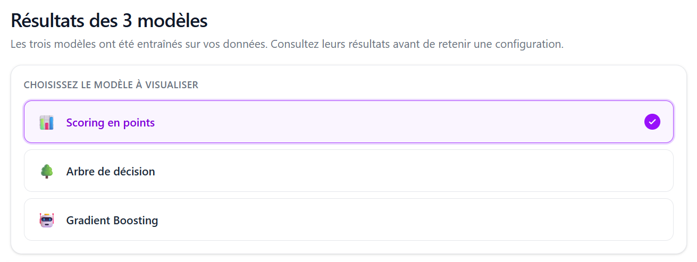
\includegraphics[width=0.9\textwidth]{images/chapitre5/3modeles.png}
    \caption{Affichage de l'Agent IA pour le choix de modélisation (à renseigner par l'utilisateur)}
    \label{fig:choix-modelisation}
\end{figure}

Une présentation et analyse des résultats de chaque modèle est proposée ci-dessous.

% ==============================================================
\section{Scoring en points}
% ==============================================================

Sur la base de sinistre transmise, l'Agent IA va à présent appliquer un \textit{\textbf{modèle de \textit{scoring} en points}}.

\begin{figure}[H]
    \centering
    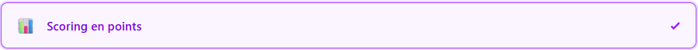
\includegraphics[width=0.9\textwidth]{images/chapitre5/points/choix_point.png}
    \label{fig:choix-point}
\end{figure}

A noter que pour faciliter l'interprétation des scores obtenus et leur passage en probabilité de fraude, nous avons demandé à l'agent de normaliser le barème de score de manière à ce que l'ensemble des combinaisons possibles soient comprises entre 0 et 1000 points.

% --------------------------------------------------------------
\subsection{Résultats du modèle}
% --------------------------------------------------------------

La construction d'un modèle de \textit{scoring} performant repose en amont sur une sélection rigoureuse des variables explicatives. Cette étape poursuit un double objectif : d'une part, retenir uniquement les variables porteuses d'un pouvoir discriminant réel vis-à-vis de la variable cible (l'occurrence de fraude), afin de maximiser la performance prédictive du modèle ; d'autre part, garantir la parcimonie du barème, condition essentielle à sa lisibilité, à son appropriation par les gestionnaires sinistres et à sa maintenabilité dans le temps.

Un barème surchargé de critères, même statistiquement significatifs, perd en effet en opérationnalité et devient difficilement auditable.

Une fois la phase de sélection des variables terminée, un nombre de points est affecté à chaque modalité ou situation à risque. Plus une modalité est associée historiquement à un niveau élevé de fraude, plus le nombre de points attribué est important. À l'inverse, les situations jugées peu suspectes reçoivent peu de points, voire aucun.

Le \textit{scoring} en points repose donc sur une logique additive : chaque dossier cumule des points selon les caractéristiques qu'il présente. Le barème reflète ainsi la contribution relative de chaque critère au risque de fraude.

En sortie du modèle, on obtient les indicateurs suivants :

\begin{itemize}[label=$\bullet$]
    \item Le nombre de variables retenues dans le modèle de \textit{scoring} (20) ;
    \item Pour chaque variable, le nombre de points associé à chaque modalité ;
    \item «~Effectif train~» correspondant au nombre de lignes de chaque modalité au sein de la base d'apprentissage ;
    \item «~Taux de fraude train~», le taux de fraude observé sur la base d'apprentissage ;
    \item Le WOE (Weight of Evidence), qui correspond au log-odds de la modalité, recentré sur le log-odds global :
\end{itemize}

\begin{equation}
    \text{WOE} = \ln(\text{odds}_{\text{modalité}}) - \ln(\text{odds}_{\text{global}})
\end{equation}

\textcolor{vert}{Par exemple, pour la variable « \textit{repaired\_avg\_invoice\_vs\_market} », sur la modalité « Off market », le taux global de fraude est de $2\,752 / 24\,000 \approx 11,5~\%$, donc $\ln(0,48 / 0,52) - \ln(0,115 / 0,885) = 1,96$}. Un WOE positif signifie donc « plus risqué que la moyenne du portefeuille », négatif « moins risqué », et 0 correspond exactement au risque moyen. C'est la variable explicative réellement injectée dans la régression : chaque modalité est remplacée par son WOE.

\begin{itemize}[label=$\bullet$]
    \item L'Information Value (IV) : c'est une mesure de pouvoir discriminant univarié, indépendante du modèle final, donnée par :
\end{itemize}

\begin{equation}
    \text{IV} = \sum_{\text{modalités}} (\%\,\text{fraudes} - \%\,\text{non-fraudes}) \times \text{WOE}
\end{equation}

\textcolor{vert}{Par exemple, sur la variable «\textit{repaired\_avg\_invoice\_vs\_market} » : $(0,661 - 0,953) \times (-0,366) + (0,339 - 0,048) \times 1,965 = 0,680$.}

\begin{table}[H]
    \centering
    \renewcommand{\arraystretch}{1.3}
    \begin{tabularx}{0.7\textwidth}{|>{\raggedright\arraybackslash}X|>{\raggedright\arraybackslash}X|}
        \hline
        \rowcolor{accenture}
        \textcolor{white}{\textbf{Valeur de l'IV}} & \textcolor{white}{\textbf{Interprétation}} \\
        \hline
        $< 0,02$ & Inutile \\
        \hline
        $0,02 - 0,1$ & Faible \\
        \hline
        $0,1 - 0,3$ & Moyen \\
        \hline
        $0,3 - 0,5$ & Fort \\
        \hline
        $> 0,5$ & À examiner \\
        \hline
    \end{tabularx}
    \caption{Grille d'interprétation de l'IV}
    \label{tab:interpretation-iv}
\end{table}

\begin{itemize}[label=$\bullet$]
    \item Le coefficient logistique : c'est le coefficient de la variable WOE-isée dans la régression multivariée. Sa référence naturelle est 1 : si une variable était seule dans le modèle, son coefficient vaudrait mécaniquement 1 puisque le WOE est déjà exprimé en log-odds. Les valeurs retournées par le modèle (ici 0,997 / 0,980 / 0,980 / 0,904) sont donc à lire comme un facteur d'atténuation. S'il est proche de 1, cela signifie que la variable apporte une information peu redondante avec les autres. À noter que le 0,904 de « \textit{vehicle\_market\_value} » indique un léger recouvrement avec d'autres variables du modèle. Les signaux d'alerte seraient un coefficient très inférieur à 1 (redondance forte), supérieur à 1,3--1,5, ou négatif, ce dernier cas traduisant une inversion de sens due à de la colinéarité.
    \item La stabilité de la variable : elle représente la fréquence de sélection de la variable sur des rééchantillonnages (\textit{bootstrap} ou validation croisée). La valeur 1 indique que la variable est systématiquement retenue.
\end{itemize}

\begin{figure}[H]
    \centering
    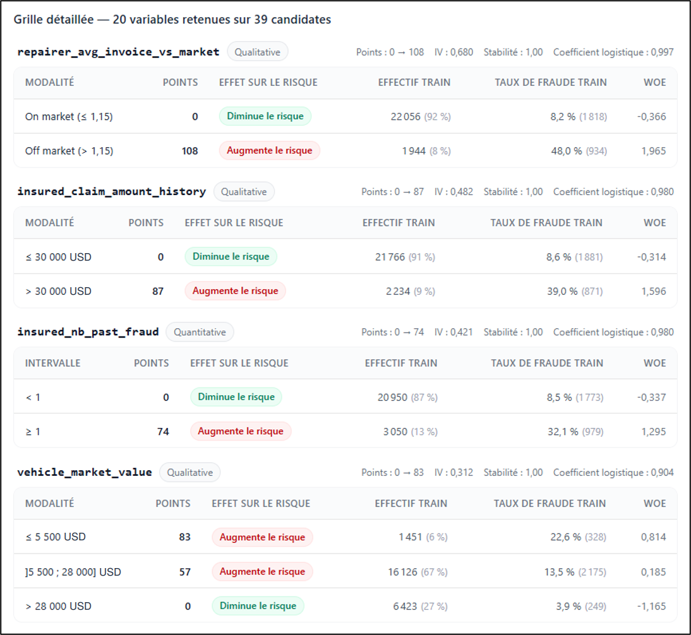
\includegraphics[width=0.9\textwidth]{images/chapitre5/points/grille_points.png}
    \caption{Extrait de la grille d'attribution des points du modèle de \textit{scoring} en points}
    \label{fig:grille-points}
\end{figure}

Les résultats du modèle de \textit{scoring} permettent de distinguer 3 catégories d'indicateurs :

\begin{itemize}[label=$\bullet$]
    \item En premier lieu, les signaux forts correspondent aux variables les plus discriminantes, historiquement associées à un sur-risque de fraude et donc fortement pondérées.
    \begin{itemize}[label=$\circ$]
        \item Le ratio facture/marché du réparateur domine le barème : une facture supérieure de 15~\% au prix de marché (« off market ») atteint un taux de fraude de 48,0~\% (contre 11,5~\% en moyenne) et se voit attribuer le maximum de 108 points, pour une IV de 0,680.
        \item Viennent ensuite l'historique des montants réclamés par l'assuré (un cumul supérieur à 30\,000 USD porte le taux de fraude à 39,0~\% et vaut 87 points) ;
        \item Les antécédents de fraude de l'assuré (au moins une fraude passée : 32,1~\% de fraude, 74 points) ;
        \item Et la valeur marchande du véhicule (un véhicule de moins de 5\,500~\euro{} atteint 22,6~\% de fraude, 83 points).
    \end{itemize}
\end{itemize}

\noindent\textbf{Ces quatre variables concentrent l'essentiel du pouvoir discriminant du modèle.}

\begin{itemize}[label=$\bullet$]
    \item En deuxième lieu, les signaux moyens sont des indicateurs plus diffus, moins déterminants pris isolément, mais dont le cumul affine sensiblement l'évaluation du risque. On y retrouve le nombre d'amendements à la déclaration (jusqu'à 67 points pour au moins trois modifications, 26,3~\% de fraude), l'âge du véhicule (49 points au-delà de neuf ans), le nombre de sinistres passés du véhicule comme de l'assuré, le nombre de contrats actifs, le délai depuis le dernier sinistre (64 points en deçà de 800 jours) ou encore les changements récents d'adresse. Chacun pèse modérément, mais leur accumulation sur un même dossier peut faire fortement grimper le score final.
    \item En troisième lieu, la logique du barème intègre des modalités protectrices, auxquelles zéro ou très peu de points sont attribués afin d'éviter une surévaluation du risque. Ainsi, un dossier où la police a été contactée ne reçoit aucun point, contre 60 points en l'absence de toute autorité ; la présence d'au moins un témoin annule les 38 points attribués à un dossier sans témoin ; de même, un véhicule de plus de 28\,000 USD, un contrat de plus de trois ans ou un assuré de plus de 24 ans ne contribuent pas au score. Ces situations, statistiquement associées à un moindre risque de fraude, viennent naturellement contrebalancer les signaux aggravants.
    \item Enfin, on notera la présence de variables faiblement discriminantes conservées dans le barème mais au poids marginal, comme la profession de l'assuré (IV de 0,022) ou le canal de déclaration : elles n'apportent qu'un ajustement mineur au score et confirment, à l'inverse, la prééminence des signaux liés au réparateur et aux antécédents de l'assuré.
\end{itemize}

Dans l'ensemble, ce barème repose sur une logique transparente et interprétable, combinant expertise métier et observations empiriques, afin de produire un score global reflétant le niveau de suspicion de fraude associé à chaque dossier.

On peut également s'intéresser à l'importance relative des variables dans le modèle de prédiction de fraude, qui doit intuitivement être liée à l'attribution des points dans le modèle de \textit{scoring} :

\begin{figure}[H]
    \centering
    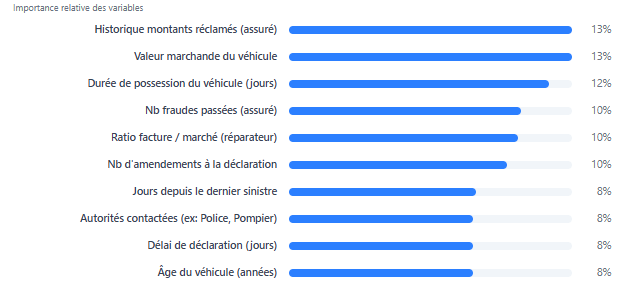
\includegraphics[width=0.9\textwidth]{images/chapitre5/points/importance_variables_points.png}
    \caption{Hiérarchie de l'importance globale des variables dans le modèle de \textit{scoring} en points}
    \label{fig:importance-variables-points}
\end{figure}

On remarque que l'importance des variables est ici relativement répartie, mais avec une hiérarchie nette : le pouvoir explicatif s'étale de 2~\% à 11~\%, sans qu'aucune variable n'écrase les autres, tout en laissant émerger un petit groupe de signaux dominants.

En tête figure le ratio facture/marché du réparateur (11~\%), suivi de l'historique des montants réclamés par l'assuré (9~\%), de la valeur marchande du véhicule (8~\%), du nombre de fraudes passées et du nombre d'amendements à la déclaration (7~\% chacun). À l'autre extrémité, des variables comme la profession de l'assuré, le canal de déclaration ou le ratio de surévaluation ne pèsent chacune que 2~\%.

Cette hiérarchie relativement douce est cohérente avec la nature même du \textit{scoring} en points : reposant sur une agrégation additive de nombreux critères, le modèle répartit le risque sur un large ensemble de signaux plutôt que de le concentrer sur quelques-uns. C'est là une force autant qu'une caractéristique : le modèle ne dépend pas excessivement d'une seule variable, ce qui le rend robuste et stable (son PSI très faible et l'absence de surapprentissage le confirment) et lui permet de conserver sa pertinence même lorsqu'une variable est absente d'un dossier de sinistre.

On note enfin que les variables présentant les plus fortes importances sont aussi celles susceptibles d'attribuer le plus grand nombre de points dans le barème : le ratio facture/marché, qui domine ce classement, est également la variable la mieux dotée de la grille (jusqu'à 108 points). Cette cohérence entre poids dans la grille et importance dans le score global est logique, puisque l'importance mesure précisément la part de l'amplitude totale de points qu'une variable peut faire varier.

Ces observations sont en accord avec l'étude de fréquence réalisée en amont du lancement du modèle (cf. \ref{subsec:analyse-frequence}).

Le modèle est ensuite appliqué à l'ensemble de la base sinistres : pour chaque dossier, les points associés aux caractéristiques observées sont additionnés, produisant un score global de suspicion qui synthétise le niveau de risque du sinistre. Plus ce score est élevé, plus le dossier présente un profil proche de celui des sinistres historiquement identifiés comme frauduleux.

Une fois les scores calculés, il est important de regarder leur distribution par classe (histogrammes superposés) de fraudeurs/non fraudeurs : visuellement, plus les deux distributions sont \textbf{séparées}, meilleur est le modèle.

\begin{figure}[H]
    \centering
    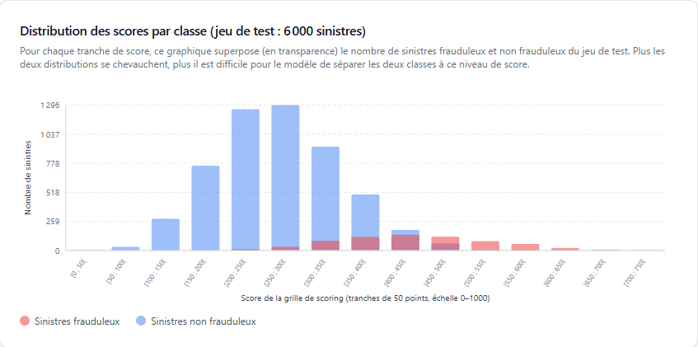
\includegraphics[width=0.9\textwidth]{images/chapitre5/points/distribution_points.png}
    \caption{Distribution des scores par classe (fraudeur/non fraudeur)}
    \label{fig:distribution-points}
\end{figure}

On observe sur la figure~\ref{fig:distribution-points} que les sinistres frauduleux sont principalement concentrés sur la droite du graphique, correspondant aux scores élevés, à l'inverse des sinistres non frauduleux qui sont concentrés à gauche.

L'analyse de la sortie du modèle ne se limite pas à la distribution des scores par classe. Il convient également de comparer les niveaux de score observés entre les sinistres frauduleux et les sinistres non frauduleux. Si le modèle est pertinent, les dossiers frauduleux doivent, en moyenne, présenter des scores plus élevés. Cette étape permet d'évaluer la capacité du \textit{scoring} à séparer les deux populations et à hiérarchiser le risque de fraude de manière cohérente.

\begin{figure}[H]
    \centering
    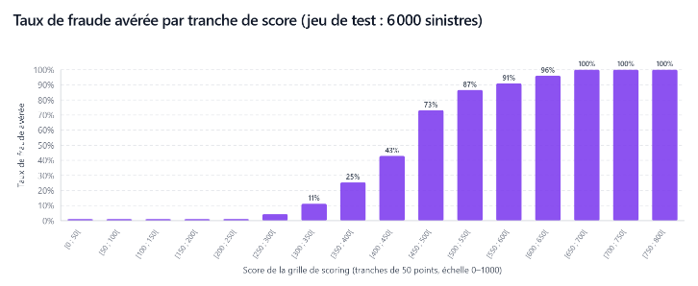
\includegraphics[width=0.9\textwidth]{images/chapitre5/points/taux_fraude_averee_points.png}
    \caption{Taux de fraude avérée par tranche de score de suspicion}
    \label{fig:taux-fraude-points}
\end{figure}

À noter que les figures~\ref{fig:distribution-points} et~\ref{fig:taux-fraude-points} mesurent la qualité prédictive sur le jeu de test, c'est-à-dire sur des sinistres dont le modèle n'a pas eu connaissance lors de sa phase d'apprentissage. Les indicateurs reflètent donc sa capacité de généralisation à de nouveaux dossiers, et non une simple performance sur les données d'entraînement.

La figure~\ref{fig:taux-fraude-points} met ici en évidence une relation croissante par paliers entre le score de suspicion et le taux de fraude avérée, ce qui confirme la capacité du modèle à discriminer efficacement les dossiers selon leur niveau de risque : plus le score est élevé, plus la probabilité de fraude augmente.

À partir de la distribution des scores et de la capacité discriminante du modèle, des seuils opérationnels peuvent être définis. Ces seuils permettent de transformer un score continu en règle de gestion. Par exemple, un score faible peut correspondre à une absence de recherche complémentaire, un score intermédiaire à une investigation légère, et un score élevé à une recherche approfondie. Le choix de ces seuils repose sur un arbitrage actuariel et opérationnel entre le coût des contrôles, le nombre de faux positifs acceptables et le gain attendu en matière de fraude détectée.

Dans notre exemple, on observe une première cassure autour de 350 points, à partir de laquelle le taux de fraude avérée augmente légèrement : ce premier changement de régime justifie le déclenchement d'une investigation légère. Une seconde cassure apparaît autour de 450 points, où le taux de fraude avérée croît nettement, seuil à partir duquel une investigation approfondie se justifie.

Autrement dit, les règles d'investigation suivantes peuvent être mises en place :

\begin{itemize}[label=$\bullet$]
    \item \textcolor{vert}{Score compris entre 0 et 350 : pas d'investigation}
    \item \textcolor{orange}{Score compris entre 350 et 450 : investigation légère}
    \item \textcolor{rouge}{Score supérieur à 450 : investigation poussée}
\end{itemize}

Enfin, si l'on considère les sinistres classifiés comme nécessitant une investigation poussée comme « frauduleux » (score supérieur à 450), le score étant construit sur une échelle de 0 à 1\,000 points, un seuil de 450 points équivaut à  45~\% de l'échelle ; c'est cette normalisation qui permet d'exprimer le seuil de décision en pourcentage dans la matrice de confusion. Dans notre choix graphique ci-dessus, on obtient la matrice de confusion suivante :

\begin{figure}[H]
    \centering
    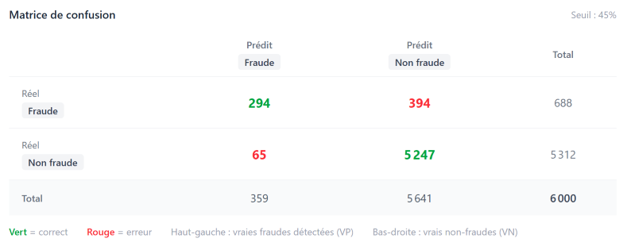
\includegraphics[width=0.9\textwidth]{images/chapitre5/points/matrice_45_points.png}
    \caption{Matrice de confusion du modèle de \textit{scoring} en points pour un seuil de 45~\%}
    \label{fig:matrice-45-points}
\end{figure}

\underline{Cette matrice permet de calculer} :

\begin{itemize}[label =$\bullet$]
    \item Le taux de non-fraudes bien classées (prédit non-fraudes / réel non-fraude total) : $5\,247 / 5\,312 = 98{,}77~\%$ ;
    \item Le taux de fraude détectées (prédit fraude / réel fraude) : $294 / 688 = 42{,}73~\%$.
    \item Le taux de sinistres signalés frauduleux : prédit fraude / total = $359 / 6\,000 = 5{,}98~\%$.
\end{itemize}

Néanmoins, la méthode graphique de détermination du seuil n'est pas toujours la meilleure et une \textbf{optimisation du seuil} afin d'obtenir la meilleure qualité de modèle est proposée dans le passage suivant.

% --------------------------------------------------------------
\subsection{Qualité du modèle obtenu}
\label{sec:qualite-modele}
% --------------------------------------------------------------

Les indicateurs présentés dans cette partie sont l'application pratique des critères de qualité des modèles présentés en section~\ref{sec:criteres-evaluation}.

Pour commencer, un point de vigilance mérite d'être souligné concernant le \textbf{choix du seuil de décision}. Le modèle ne restitue pas une classification binaire mais une probabilité de fraude ; il convient donc de fixer un seuil au-delà duquel un sinistre est considéré comme frauduleux. Le seuil de 0,5, retenu par méthode graphique, se révèle en réalité inadapté aux données fortement déséquilibrées : avec seulement 11,5~\% de fraudes, la majorité des scores se concentrent sous 0,45, si bien que le modèle ne détecte qu'une fraction infime des fraudes réelles.

Pour corriger ce biais, on recourt à l'\textbf{indice de Youden}, défini comme :

\begin{equation}
    J = \text{Sensibilité} + \text{Spécificité} - 1
\end{equation}

Cet indice identifie le seuil qui maximise l'écart entre le taux de vrais positifs (fraudes correctement détectées) et le taux de faux positifs (non-fraudes signalées à tort) ; il correspond graphiquement au point de la courbe ROC le plus éloigné de la diagonale du hasard, c'est-à-dire celui où le modèle sépare le mieux les deux populations.

Appliqué à ce modèle, le seuil optimal est alors de 35~\%.

\underline{Les résultats du modèle obtenus avec l'utilisation de ce seuil sont présentés ci-dessous} :

\begin{figure}[H]
    \centering
    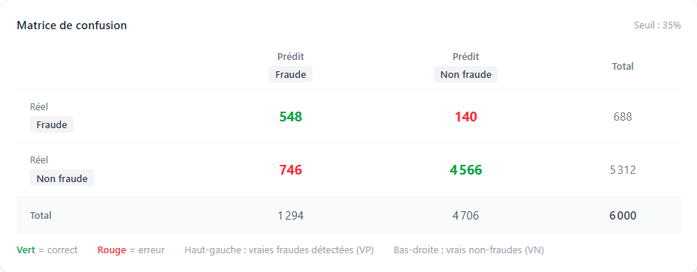
\includegraphics[width=0.9\textwidth]{images/chapitre5/points/matrice_optimal_points.png}
    \caption{Matrice de confusion au seuil optimal du modèle de \textit{scoring} en points (35~\%)}
    \label{fig:matrice-optimal-points}
\end{figure}

\underline{Cette matrice permet de calculer} :

\begin{itemize}
    \item Le taux de non-fraudes bien classées (prédit non-fraudes / réel non-fraude total) : $4\,732 / 5\,312 = 89{,}08~\%$ ;
    \item Le taux de fraude détectées (prédit fraude / réel fraude) : $527 / 688 = 76{,}60~\%$ ;
    \item Le taux de sinistres signalés frauduleux : prédit fraude / total = $1\,107 / 6\,000 = 18{,}45~\%$.
\end{itemize}

L'efficacité opérationnelle de l'outil se mesure aussi à sa capacité à concentrer la fraude dans un volume restreint de dossiers à investiguer. Au seuil retenu, le modèle signale 18,45~\% des sinistres, parmi lesquels 76,42~\% sont réellement frauduleux, soit une densité de fraude environ 6,6 fois supérieure à celle d'un contrôle aléatoire. L'outil permet ainsi aux gestionnaires de concentrer leurs efforts sur un sous-ensemble à forte valeur, plutôt que de traiter l'ensemble du portefeuille.
%calcul du 6,6 : 76,42 / 11,5 = 6,6

\underline{À présent, observons les autres indicateurs de qualité du modèle} :

\begin{figure}[H]
    \centering
    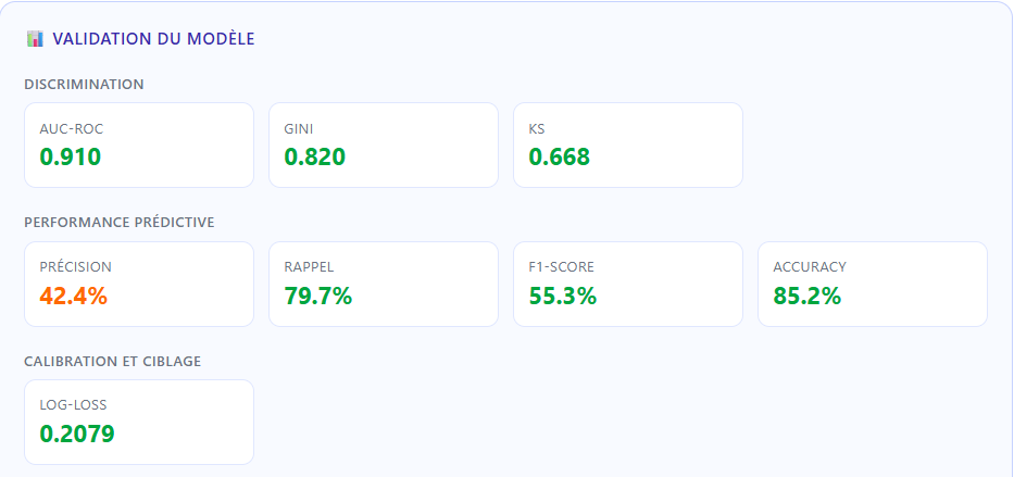
\includegraphics[width=0.9\textwidth]{images/chapitre5/points/synthese_points.png}
    \caption{Synthèse des métriques de performance et de stabilité du modèle de \textit{scoring} en points}
    \label{fig:synthese-points}
\end{figure}

\begin{figure}[H]
    \centering
    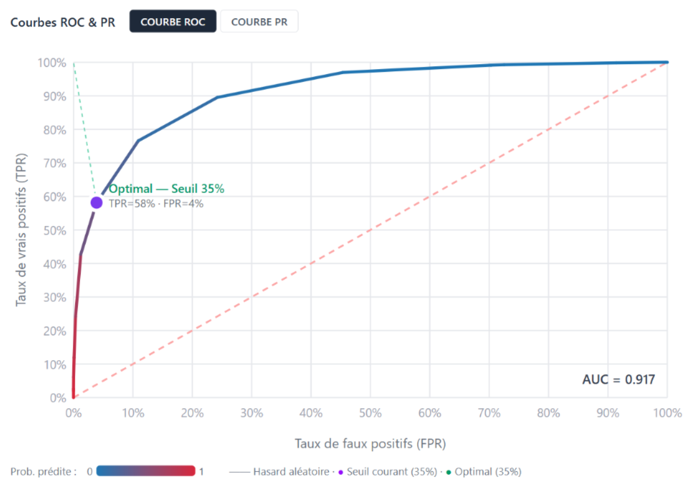
\includegraphics[width=0.9\textwidth]{images/chapitre5/points/courbe_roc_auc_points.png}
    \caption{Courbe ROC et AUC correspondant au modèle de \textit{scoring} en points}
    \label{fig:roc-points}
\end{figure}

En retenant le seuil optimal de 35~\%, les indicateurs obtenus s'interprètent de la façon suivante :

\begin{itemize}[label = $\bullet$]
    \item \textbf{AUC-ROC (0,917)} : excellente capacité de discrimination, très au-dessus du seuil de 0,8 considéré comme bon ; le modèle sépare efficacement fraudeurs et non-fraudeurs.
    \item \textbf{Gini (0,835)} : cohérent avec l'AUC, ce niveau traduit un pouvoir discriminant élevé, largement supérieur aux standards habituels en assurance.
    \item \textbf{KS (0,666)} : bien au-delà du seuil de 0,5, il confirme une nette séparation entre les distributions de scores des deux populations.
    \item \textbf{Précision (47,6~\%)} : parmi les dossiers signalés comme frauduleux, un peu plus de quatre sur dix le sont réellement. Valeur modérée, mais attendue à ce seuil abaissé et acceptable au vu de l'objectif de détection.
    \item \textbf{Rappel (76,6~\%)} : le modèle détecte près de quatre fraudes sur cinq, ce qui est le point fort de ce seuil et l'objectif prioritaire en détection de fraude.
    \item \textbf{F1-score (58,7~\%)} : compromis honnête entre précision et rappel, en nette amélioration par rapport au seuil de 0,5.
    \item \textbf{Accuracy (87,6~\%)} : taux de bonnes classifications élevé, à interpréter toutefois avec prudence sur données déséquilibrées où cet indicateur est peu informatif à lui seul.
    \item \textbf{Log-loss (0,2015)} : valeur faible, signe d'une bonne calibration des probabilités prédites.
\end{itemize}

Dans l'ensemble, le modèle présente d'excellents indicateurs de discrimination et de stabilité ; le seul point de vigilance concerne la précision modérée, contrepartie assumée d'un rappel volontairement élevé.

Ces résultats sont cohérents avec la nature du modèle : sa simplicité et sa parcimonie le rendent naturellement robuste et peu sujet au surajustement.

\underline{Enfin, concernant les indicateurs de robustesse et stabilité du modèle, les résultats suivants sont obtenus} :

\begin{itemize}[label = $\bullet$]
    \item \textbf{Backtesting (écart AUC train/test de 0,003)} : écart quasi nul entre apprentissage et test, confirmant l'absence de surapprentissage et une bonne capacité de généralisation.
    \item \textbf{PSI (0,0026)} : très inférieur à 0,1, il atteste d'une parfaite stabilité de la distribution des scores.
\end{itemize}

\begin{figure}[H]
    \centering
    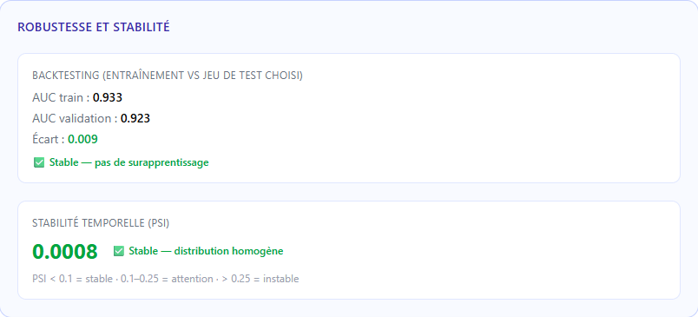
\includegraphics[width=0.9\textwidth]{images/chapitre5/points/robustesse_points.png}
    \caption{Indicateurs de robustesse et de stabilité du modèle de \textit{scoring} en points}
    \label{fig:robustesse-points}
\end{figure}

% --------------------------------------------------------------
\subsection{Limites et précautions d'interprétation}
% --------------------------------------------------------------

% ==============================================================
\section{Arbre de décision}
% ==============================================================

Cette section présente l'utilisation de la modélisation via un « arbre de décision » pour estimer la probabilité de fraude.

\begin{figure}[H]
    \centering
    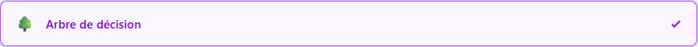
\includegraphics[width=0.9\textwidth]{images/chapitre5/arbre/arbre.png}
    \label{fig:choix-arbre}
\end{figure}

% --------------------------------------------------------------
\subsection{Résultats du modèle}
% --------------------------------------------------------------

\textit{TROUVER UNE LIMITE}


L'arbre construit admet les paramètres suivants :

\begin{itemize}[label = $\bullet$]
    \item Profondeur : 5
    \item Feuilles : 68
    \item Nœuds internes : 67
\end{itemize}

L'arbre construit admet les caractéristiques structurelles suivantes :

\begin{itemize}[label = $\bullet$]
    \item \textbf{La profondeur (5)}, qui correspond au nombre maximal de niveaux de décision successifs entre la racine de l'arbre et ses feuilles. Concrètement, un dossier traverse au plus cinq coupures successives (cinq questions posées sur ses variables) avant d'aboutir à une prédiction. Cette profondeur a été volontairement limitée à 5 : un arbre trop profond mémoriserait les particularités de l'échantillon d'apprentissage (sur-apprentissage) et généraliserait mal à de nouveaux dossiers, tandis qu'un arbre trop peu profond serait incapable de capter les interactions entre variables. Une profondeur de 5 constitue ainsi un compromis entre pouvoir de discrimination et capacité de généralisation.
    \item \textbf{Les feuilles (68)} sont les nœuds terminaux de l'arbre, c'est-à-dire les points d'aboutissement où une décision finale est rendue (dossier classé frauduleux ou non). Chaque feuille regroupe un ensemble de dossiers partageant le même parcours de décision, et se voit attribuer une probabilité de fraude correspondant à la proportion de fraudes observée parmi les dossiers d'apprentissage qui y aboutissent. L'arbre compte ici 68 feuilles, soit 68 profils de risque distincts.
    \item \textbf{Les nœuds internes (67)} sont les points de décision situés avant les feuilles : à chaque nœud interne, l'arbre applique un test sur une variable (par exemple « le réparateur est-il signalé ? » ou « le montant réclamé dépasse-t-il un certain seuil ? ») qui oriente le dossier vers l'une ou l'autre branche. Le nombre de nœuds internes est directement lié au nombre de feuilles : un arbre binaire comportant 68 feuilles possède nécessairement 67 nœuds internes.
\end{itemize}

\begin{figure}[H]
    \centering
    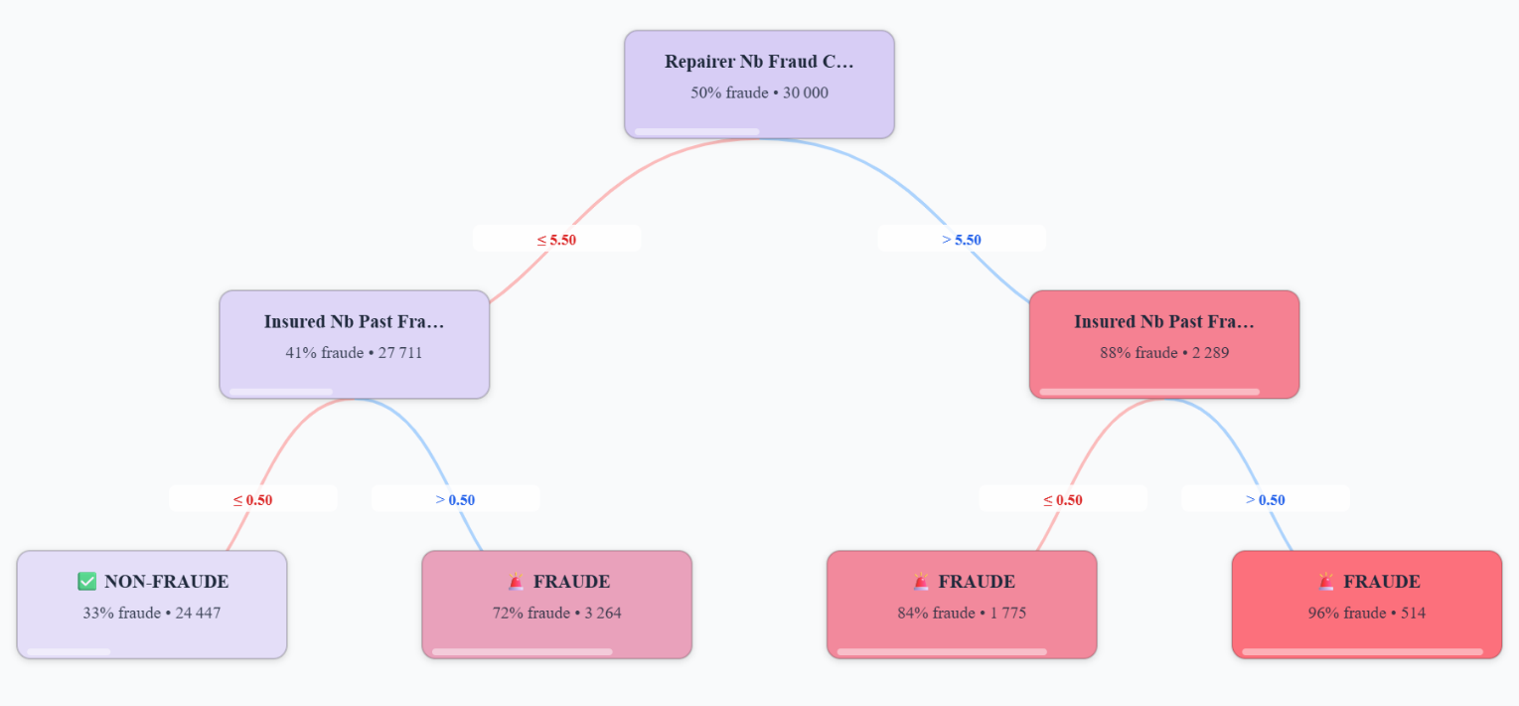
\includegraphics[width=0.9\textwidth]{images/chapitre5/arbre/representation_visuelle_arbre.png}
    \caption{Représentation visuelle de l'arbre avec un découpage sur une profondeur de 2 branches (5 branches au total)}
    \label{fig:representation-arbre}
\end{figure}

On peut également s'intéresser à l'importance relative des variables dans le modèle de prédiction de fraude, qui doit intuitivement être liée à leur niveau et fréquence d'apparition dans l'arbre retourné :

\begin{figure}[H]
    \centering
    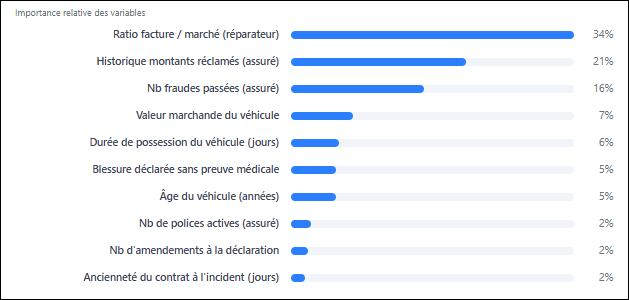
\includegraphics[width=0.9\textwidth]{images/chapitre5/arbre/importance_variables_arbre.png}
    \caption{Hiérarchie de l'importance globale des variables dans le modèle "arbre de décision"}
    \label{fig:importance-variables-arbre}
\end{figure}

Le profil d'importance de l'arbre de décision est ici assez réparti, sans variable dominante isolée. 
Trois critères arrivent en tête à égalité, chacun structurant 14~\% des décisions de l'arbre : le ratio facture/marché du réparateur, l'historique des montants réclamés par l'assuré et le nombre de fraudes passées de l'assuré.

Ils sont suivis de près par l'âge du véhicule et la présence d'une blessure déclarée sans preuve médicale (12~\% chacun), puis par le nombre d'amendements à la déclaration (10~\%) et le nombre de sinistres passés du véhicule (9~\%). Ce n'est qu'ensuite que les autres variables voient leur poids décroître nettement, jusqu'à devenir marginales (2~\% ou moins pour l'ancienneté du contrat, les autorités contactées ou le nombre de véhicules impliqués).

On notera par ailleurs que les variables absentes de ce graphique présentent une importance nulle : elles n'ont tout simplement jamais été retenues comme critère de coupure par l'arbre. Ce phénomène s'explique par la structure même du modèle, dont la profondeur a été limitée à 5 niveaux : \textbf{avec seulement 67 nœuds internes disponibles, l'arbre concentre ses coupures sur les variables les plus discriminantes et n'a pas l'occasion de mobiliser les autres, qui restent inexploitées.}

Cette répartition indique que l'arbre construit ses coupures successives sur un ensemble relativement large de variables, plutôt que de faire reposer sa structure sur un ou deux critères dominants. On retrouve néanmoins \textbf{en tête les mêmes signaux forts que dans les autres modèles} (ratio facture/marché, historique de l'assuré, antécédents de fraude), ce qui rejoint directement l'analyse de fréquence de fraude où ces variables ressortaient déjà comme les plus discriminantes. La cohérence entre modèles renforce la confiance dans la pertinence de ces résultats.

Il faut toutefois noter que cette mesure d'importance renseigne sur la manière dont l'arbre est structuré (la part des sinistres traités par les nœuds utilisant chaque variable), et non directement sur sa capacité de généralisation. L'arbre de décision demeure en effet le modèle le plus exposé au surapprentissage, comme le montre l'écart un peu plus marqué entre son AUC d'entraînement et son AUC de validation (cf. plus bas): sa structure s'ajuste finement aux données observées, au risque de manquer de robustesse sur les cas moins typiques.

L'agent retourne une représentation visuelle complète de l'arbre créé mais également d'autres graphiques\footnote{Graphiques réalisés sur la base de l'échantillon test (6\,000 lignes) et non sur l'échantillon d'apprentissage du modèle.}, tels que la distribution des scores par classe (histogrammes superposés) : distribution du score des fraudeurs vs distribution du score des non-fraudeurs. Comme pour le modèle de \textit{scoring} en points, visuellement, plus les deux distributions sont \textbf{séparées}, meilleur est le modèle.

\begin{figure}[H]
    \centering
    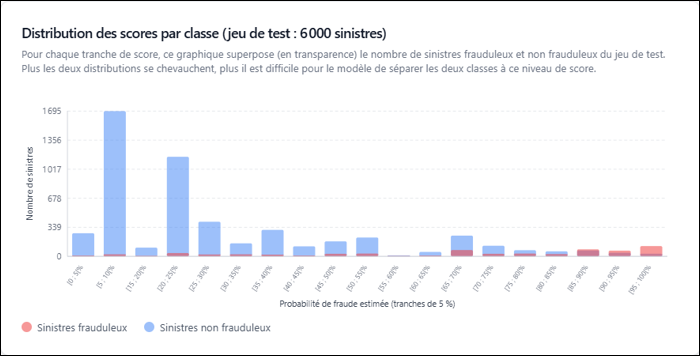
\includegraphics[width=0.9\textwidth]{images/chapitre5/arbre/distribution_score_arbre.png}
    \caption{Distribution des scores par classe avec un arbre de décision (fraudeur/non fraudeur)}
    \label{fig:distribution-arbre}
\end{figure}

On observe sur ce graphique que la proportion de sinistres frauduleux (en rouge) augmente progressivement avec la probabilité estimée : quasi nulle dans les tranches basses, elle devient majoritaire dans les tranches les plus élevées ([90-100~\%]). Cette progression témoigne d'un pouvoir de discrimination réel, même si un chevauchement subsiste dans les tranches intermédiaires, et que l'on retrouve certaines fraudes avec des probabilités pourtant faibles, ce qui témoigne d'un défaut du modèle.

Comme pour le modèle de \textit{scoring} en points, le second graphique retourné par l'agent est le taux de fraude avéré par tranche de probabilité en sortie de l'arbre. Si le modèle est pertinent, les dossiers frauduleux doivent, en moyenne, présenter des probabilités plus élevées. Cette étape permet d'évaluer la capacité de l'arbre à séparer les deux populations et à hiérarchiser le risque de fraude de manière cohérente.

\begin{figure}[H]
    \centering
    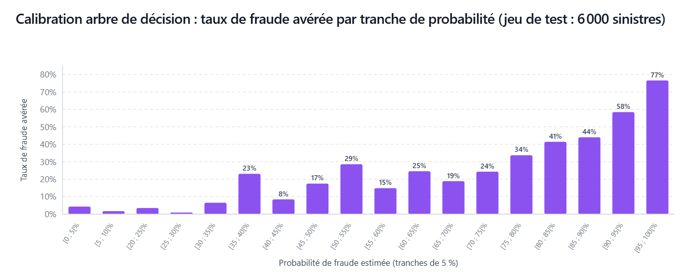
\includegraphics[width=0.9\textwidth]{images/chapitre5/arbre/taux_fraude_averee_arbre.png}
    \caption{Taux de fraude avérée par tranche de score de suspicion}
    \label{fig:taux-fraude-arbre}
\end{figure}

La sortie issue de l'arbre de décision met en évidence une relation claire et structurée entre la probabilité de fraude estimée par le modèle et le taux de fraude réellement observé. On observe une \textbf{progression à tendance croissante du taux de fraude} à mesure que la probabilité prédite augmente, ce qui traduit une bonne capacité du modèle à ordonner les dossiers selon leur niveau de risque. Les premières tranches de probabilité (faibles scores) présentent des taux de fraude très limités, tandis que les tranches les plus élevées concentrent une proportion significativement plus importante de fraudes, pouvant dépasser 75~\%.

Cette montée progressive est particulièrement intéressante d'un point de vue opérationnel, car elle permet de \textbf{segmenter efficacement les dossiers} et de prioriser les investigations sur les cas les plus risqués.

Par ailleurs, les caractéristiques du modèle (profondeur maximale de 5) traduisent un compromis maîtrisé entre complexité et capacité de généralisation. Le modèle reste suffisamment lisible tout en capturant des patterns discriminants. En synthèse, cette sortie confirme que l'arbre de décision fournit une \textbf{hiérarchisation cohérente et exploitable du risque de fraude}, avec une forte concentration des cas frauduleux dans les segments de probabilité élevée.

Si l'on s'appuie sur la distribution observée, l'idée est de définir des seuils qui maximisent la détection tout en restant opérationnellement soutenables (ne pas envoyer trop de dossiers en investigation lourde).

On peut distinguer \textbf{trois zones de risque} assez naturelles :

\begin{itemize}[label = $\bullet$]
    \item \textbf{Zone faible ($<$35~\%)} : le taux de fraude reste globalement modéré (inférieur à $\sim$10~\%). Ces dossiers peuvent être traités en flux standard, éventuellement avec des contrôles légers automatisés.
    \item \textbf{Zone intermédiaire ($\approx$ 35~\% à 90~\%)} : on observe une montée progressive du taux de fraude (environ 20~\% à 30~\%+) : un \textbf{seuil de vérification intermédiaire autour de 65--70~\%} paraît pertinent. À ce niveau, on commence à avoir un enrichissement significatif en fraude, tout en conservant un volume de dossiers encore gérable pour des contrôles ciblés (revue documentaire, demandes complémentaires, etc.).
    \item \textbf{Zone élevée ($>$ 90~\%)} : le taux de fraude devient nettement plus important (60~\% à plus de 70~\% sur les dernières tranches). Un \textbf{seuil de vérification poussée autour de 90~\%} est cohérent. Au-delà de ce seuil, on concentre fortement les fraudes, ce qui justifie des investigations approfondies (enquête terrain, expertise renforcée, gel du dossier, etc.).
\end{itemize}

Autrement dit, les règles d'investigation suivantes peuvent être mises en place :

\begin{itemize}[label = $\bullet$]
    \item \textcolor{vert}{Probabilité $<$ 35~\% : pas d'investigation}
    \item \textcolor{orange}{Probabilité comprise entre 35~\% et 90~\% : investigation légère}
    \item \textcolor{rouge}{Probabilité supérieure à 90~\% : investigation poussée}
\end{itemize}

Enfin, si l'on considère les sinistres classifiés comme nécessitant une investigation poussée comme « frauduleux » (score supérieur à 90 dans notre choix graphique ici), on obtient la matrice de confusion suivante :

\begin{figure}[H]
    \centering
    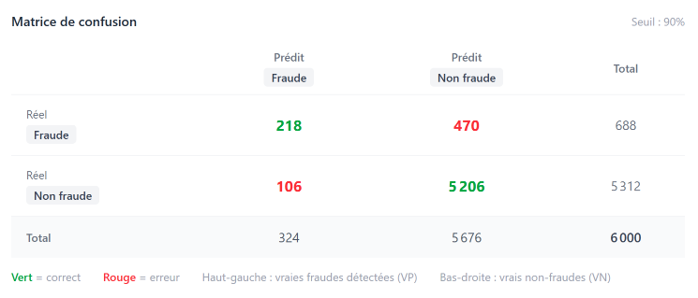
\includegraphics[width=0.9\textwidth]{images/chapitre5/arbre/matrice_confusion_90_arbre.png}
    \caption{Matrice de confusion du modèle arbre de décision pour un seuil de 90~\%}
    \label{fig:matrice-90-arbre}
\end{figure}

\underline{Cette matrice permet de calculer} :

\begin{itemize}[label = $\bullet$]
    \item Le taux de non-fraudes bien classées (prédit non-fraudes / réel non-fraude total) : $5\,206 / 5\,312 = 98{,}00~\%$ ;
    \item Le taux de fraude détectées (prédit fraude / réel fraude) : $218 / 688 = 31{,}69~\%$.
    \item Le taux de sinistres signalés frauduleux : prédit fraude / total = $324 / 6\,000 = 5{,}40~\%$.
\end{itemize}

Néanmoins, la méthode graphique de détermination du seuil n'est pas toujours la meilleure et une optimisation du seuil afin d'obtenir la meilleure qualité de modèle est proposée dans le passage suivant.

% --------------------------------------------------------------
\subsection{Qualité du modèle obtenu}
% --------------------------------------------------------------

L'introduction d'un arbre de décision permet de franchir un cap significatif. En intégrant des interactions entre variables et des effets de seuil, le modèle améliore la structuration du risque et offre une segmentation plus nette du portefeuille. La hiérarchisation des dossiers est plus cohérente : les feuilles les plus risquées de l'arbre concentrent un taux de fraude très élevé, proche de 79~\%, bien au-delà de ce que permettait le \textit{scoring} en points. Le modèle gagne ainsi en pouvoir discriminant sur les segments extrêmes, tout en conservant une certaine lisibilité grâce à sa structure arborescente.

Les indicateurs présentés dans cette partie sont l'application pratique des critères de qualité des modèles mis en place présentés en section~\ref{sec:criteres-evaluation}.

Pour commencer, on cherche le seuil optimal à partir duquel on peut considérer que les sinistres sont frauduleux à l'aide de l'indicateur de Youden\footnote{Notre agent intègre le calcul du seuil optimal dans son fonctionnement.} (présenté en section~\ref{sec:qualite-modele}). Pour le modèle utilisant des arbres de décision, le seuil optimal est de 45~\%.

\begin{figure}[H]
    \centering
    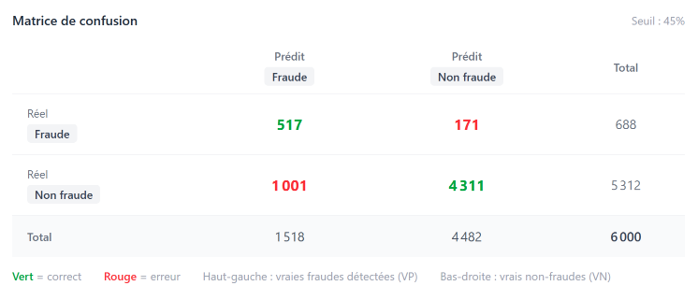
\includegraphics[width=0.9\textwidth]{images/chapitre5/arbre/matrice_confusion_optimal_45_arbre.png}
    \caption{Matrice de confusion du modèle arbre de décision au seuil optimal (45~\%)}
    \label{fig:matrice-optimal-arbre}
\end{figure}

\underline{Cette matrice permet de calculer} :

\begin{itemize}[label = $\bullet$]
    \item Le taux de non-fraudes bien classées (prédit non-fraudes / réel non-fraude total) : $4\,311 / 5\,312 = 81{,}16~\%$ ;
    \item Le taux de fraude détectées (prédit fraude / réel fraude) : $517 / 688 = 75{,}15~\%$ ;
    \item Le taux de sinistres signalés frauduleux : prédit fraude / total = $1\,518 / 6\,000 = 25{,}30~\%$.
\end{itemize}

L'efficacité opérationnelle de l'outil se mesure aussi à sa capacité à concentrer la fraude dans un volume restreint de dossiers à investiguer. Au seuil retenu, le modèle signale 25,30~\% des sinistres, parmi lesquels 75,15~\% sont réellement frauduleux, soit une densité de fraude environ 6,5 fois supérieure à celle d'un contrôle aléatoire. L'outil permet ainsi aux gestionnaires de concentrer leurs efforts sur un sous-ensemble à forte valeur, plutôt que de traiter l'ensemble du portefeuille.
%calcul du 6,5 : 75,15 / 11,5 = 6,5

\underline{À présent, observons les autres indicateurs de qualité du modèle} :

\begin{figure}[H]
    \centering
    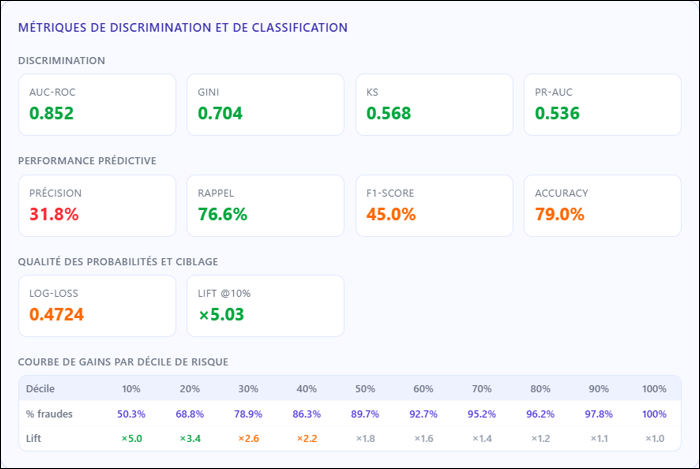
\includegraphics[width=0.9\textwidth]{images/chapitre5/arbre/synthese_metriques_arbre.png}
    \caption{Synthèse des métriques de performance et de stabilité du modèle arbre de décision au seuil 45~\%}
    \label{fig:synthese-arbre}
\end{figure}

\begin{figure}[H]
    \centering
    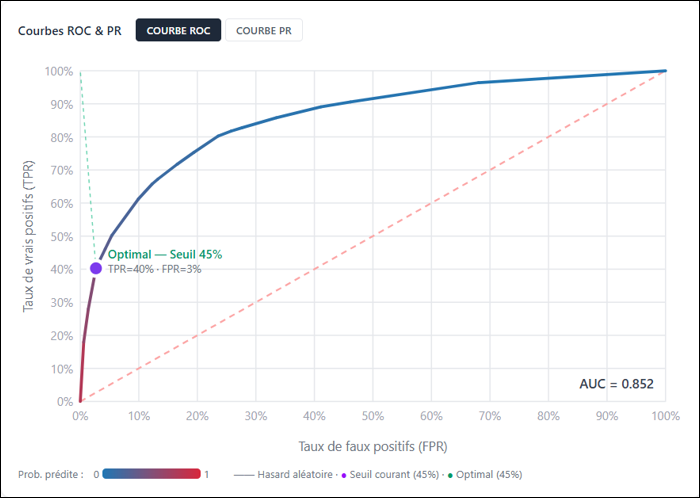
\includegraphics[width=0.9\textwidth]{images/chapitre5/arbre/courbe_roc_auc_arbre.png}
    \caption{Courbe ROC et AUC pour le modèle arbre de décision}
    \label{fig:roc-arbre}
\end{figure}

En retenant le seuil optimal de 45~\%, les indicateurs obtenus s'interprètent de la façon suivante :

\begin{itemize}[label = $\bullet$]
    \item \textbf{AUC-ROC (0,845)} : excellente capacité de discrimination, très au-dessus du seuil de 0,8 considéré comme bon ; le modèle sépare efficacement fraudeurs et non-fraudeurs.
    \item \textbf{Gini (0,690)} : cohérent avec l'AUC, ce niveau traduit un pouvoir discriminant élevé, largement supérieur aux standards habituels en assurance.
    \item \textbf{KS (0,564)} : bien au-delà du seuil de 0,5, il confirme une nette séparation entre les distributions de scores des deux populations.
    \item \textbf{Précision (34,1~\%)} : parmi les dossiers signalés comme frauduleux, un peu d'un tiers le sont réellement. Valeur modérée, mais attendue à ce seuil abaissé et acceptable au vu de l'objectif de détection.
    \item \textbf{Rappel (75,1~\%)} : le modèle détecte près de trois fraudes sur quatre, ce qui est le point fort de ce seuil et l'objectif prioritaire en détection de fraude.
    \item \textbf{F1-score (46,9~\%)} : compromis correct entre précision et rappel.
    \item \textbf{Accuracy (80,5~\%)} : taux de bonnes classifications élevé, à interpréter toutefois avec prudence sur données déséquilibrées où cet indicateur est peu informatif à lui seul.
    \item \textbf{Log-loss (0,4825)} : valeur modérée, traduisant une calibration des probabilités prédites correcte mais perfectible.
\end{itemize} 

Enfin, concernant les indicateurs de robustesse et stabilité du modèle, les résultats suivants sont obtenus :

\begin{itemize}[label = $\bullet$]
    \item \textbf{Backtesting (écart AUC train/test de 0,039)} : écart modéré entre apprentissage et test, signalant une tendance au surapprentissage mais restant contenue.
    \item \textbf{PSI (0,0026)} : très inférieur à 0,1, il atteste d'une bonne stabilité de la distribution des scores.
\end{itemize}

Ces résultats sont satisfaisants, mais restent moins bons que ceux du modèle de \textit{scoring} en points.

\begin{figure}[H]
    \centering
    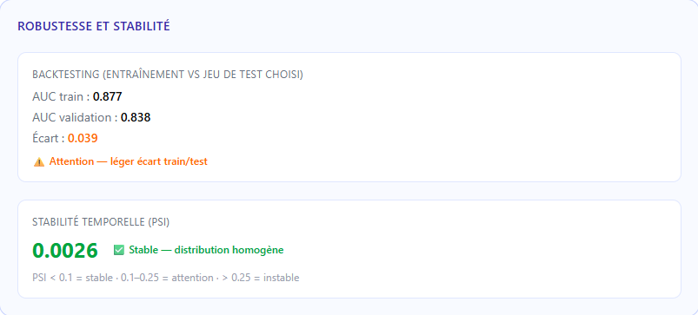
\includegraphics[width=0.9\textwidth]{images/chapitre5/arbre/robustesse_arbre.png}
    \caption{Indicateurs de robustesse et stabilité du modèle arbre de décision}
    \label{fig:robustesse-arbre}
\end{figure}

% --------------------------------------------------------------
\subsection{Limites et précautions d'interprétation}
% --------------------------------------------------------------

Les arbres de décision constituent une avancée significative par rapport aux modèles de \textit{scoring} en points, notamment par leur capacité à modéliser des interactions entre variables et à capturer des effets de seuil. Toutefois, ils présentent également un certain nombre de limites qu'il convient de considérer dans une utilisation opérationnelle.

En premier lieu, les arbres de décision sont \textbf{intrinsèquement instables} : de légères variations dans les données d'apprentissage peuvent conduire à des structures d'arbre sensiblement différentes. Cette sensibilité aux données peut impacter la robustesse du modèle et limiter sa capacité de généralisation sur de nouveaux portefeuilles. En d'autres termes, un arbre construit sur un échantillon donné peut ne pas reproduire exactement les mêmes règles de décision sur un autre échantillon pourtant similaire.

Par ailleurs, bien que les arbres permettent de capter des relations non linéaires, ils reposent sur une logique de \textbf{partitionnement par seuils successifs}, ce qui introduit des discontinuités dans la modélisation. Deux dossiers très proches peuvent ainsi être classés dans des feuilles différentes et se voir attribuer des probabilités de fraude sensiblement différentes, ce qui peut nuire à la stabilité des prédictions.

En outre, les arbres de décision ont tendance à \textbf{sur-apprendre} les données d'entraînement, en particulier lorsque leur profondeur est élevée ou que les contraintes de construction ne sont pas suffisamment strictes. Ce phénomène se traduit par une excellente performance sur les données d'apprentissage, mais une dégradation sur des données nouvelles. Des techniques de régularisation (élagage, limitation de profondeur, nombre minimal d'observations par feuille) sont donc nécessaires pour contrôler cette complexité.

Un autre point de vigilance concerne la \textbf{calibration des probabilités}. Les probabilités issues des feuilles de l'arbre (basées sur des proportions observées) peuvent être peu fiables, notamment lorsque les feuilles contiennent un nombre limité d'observations. Cela peut compliquer l'interprétation directe des scores en termes de probabilité de fraude et la définition de seuils décisionnels optimaux.

Enfin, bien que les arbres soient souvent considérés comme interprétables, cette interprétabilité peut rapidement se dégrader dès que la structure devient plus complexe (multiplication des branches et des feuilles). La lecture globale du modèle peut alors devenir difficile, en particulier pour des utilisateurs non techniques.

Ainsi, les arbres de décision offrent un bon compromis entre performance et lisibilité, mais nécessitent un encadrement méthodologique rigoureux pour garantir leur stabilité, leur robustesse et leur capacité de généralisation.

% ==============================================================
\section{Un modèle de Machine learning : le Gradient Boosting}
% ==============================================================

Enfin, le dernier modèle à être testé et dont les résultats sont présentés ci-dessous est un modèle de Machine Learning « Gradient \textit{Boosting} ».

\begin{figure}[H]
    \centering
    
\includegraphics[width=0.9\textwidth]{images/chapitre5/boost/boost.png}
    \label{fig:choix-boost}
\end{figure}

% --------------------------------------------------------------
\subsection{Résultats du modèle}
% --------------------------------------------------------------



Les paramètres du modèle de Gradient \textit{Boosting} créé sont les suivants :

\begin{itemize}[label = $\bullet$]
    \item \textbf{Le nombre d'arbres (200)} correspond au nombre de modèles élémentaires construits successivement. Dans le \textit{boosting}, chaque nouvel arbre corrige les erreurs résiduelles des précédents ; l'accumulation de 200 arbres permet d'affiner progressivement la prédiction.
    \item \textbf{La profondeur maximale (3)} limite chaque arbre à trois niveaux de coupures. Des arbres volontairement peu profonds (« arbres faibles ») sont caractéristiques du \textit{boosting} : leur pouvoir prédictif individuel est limité, mais leur combinaison séquentielle produit un modèle performant tout en réduisant le risque de surapprentissage.
    \item \textbf{Le taux d'apprentissage (0,1)} pondère la contribution de chaque arbre au modèle final. Une valeur faible ralentit l'apprentissage mais le rend plus stable et plus robuste, chaque arbre n'apportant qu'une correction mesurée.
    \item \textbf{Le sous-échantillonnage (0,8)} signifie que chaque arbre est entraîné sur 80~\% des observations, tirées aléatoirement. Cette introduction de hasard limite le surapprentissage et améliore la capacité de généralisation du modèle.
\end{itemize}

On peut également s'intéresser à l'importance relative des variables dans le modèle de prédiction de fraude :

\begin{figure}[H]
    \centering
    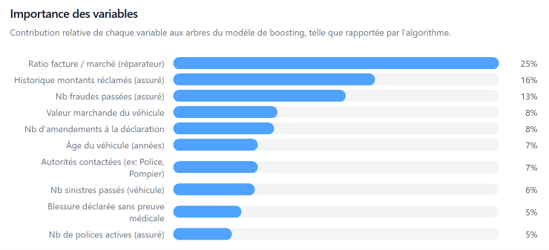
\includegraphics[width=0.9\textwidth]{images/chapitre5/boost/importance_variables_boost.png}
    \caption{Hiérarchie de l'importance globale des variables dans le modèle "Gradient Boosting"}
    \label{fig:importance-variables-boost}
\end{figure}

Le Gradient \textit{Boosting} présente un profil intermédiaire, plus équilibré que l'arbre mais toujours hiérarchisé. Le ratio facture/marché reste en tête avec 25~\%, suivi de l'historique des montants réclamés (16~\%) et du nombre de fraudes passées de l'assuré (13~\%), mais le pouvoir explicatif est ensuite mieux réparti sur une gamme plus large de variables (valeur du véhicule, amendements, durée de possession, âge du véhicule…), chacune contribuant de façon non négligeable au modèle (entre 5~\% et 8~\%).

Ce profil illustre bien ce qui fait la performance du Gradient \textit{Boosting} : en combinant de nombreux arbres construits séquentiellement, le modèle conserve la hiérarchie des signaux forts (le ratio facture/marché demeure central) tout en exploitant l'information résiduelle portée par des variables secondaires que l'arbre unique négligeait. Il réalise ainsi un compromis entre la concentration de l'arbre et la dilution du \textit{scoring}. On retrouve par ailleurs les mêmes variables clés que dans les deux autres modèles (ratio facture/marché, historique de l'assuré, antécédents de fraude) ce qui témoigne de la robustesse de ces signaux quel que soit le modèle.

Comme pour les deux autres modèles précédents, l'Agent IA retourne dans un premier temps la distribution du nombre de sinistres par tranche de 5~\% de probabilité selon l'état du sinistre (frauduleux ou non).

\begin{figure}[H]
    \centering
    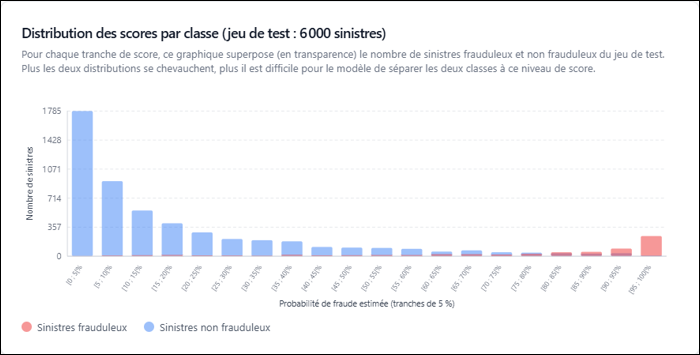
\includegraphics[width=0.9\textwidth]{images/chapitre5/boost/distribution_score_boost.png}
    \caption{Distribution des scores par classe (fraudeur/non fraudeur)}
    \label{fig:distribution-boost}
\end{figure}

Le modèle Gradient \textit{Boosting} présente une très bonne séparation des deux classes (sinistres frauduleux / non frauduleux). La grande majorité des sinistres non frauduleux se concentre dans les tranches de faible probabilité (inférieures à 30~\%) tandis que la part de sinistres frauduleux (en rouge) croît fortement dans les tranches élevées, devenant prépondérante autour des scores supérieurs à 85~\%.

Ce basculement net, ainsi que le moindre chevauchement des distributions par rapport aux deux modèles précédents confirment la supériorité du Gradient \textit{Boosting} en matière de discrimination entre dossiers frauduleux et sains.

Dans un second temps, l'Agent affiche la performance du modèle au travers de l'indicateur de taux de fraude avéré par tranche de probabilité.

\begin{figure}[H]
    \centering
    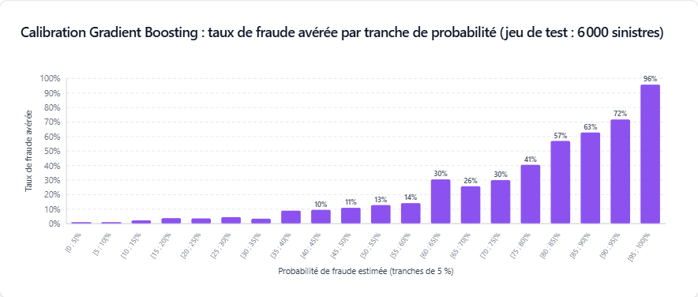
\includegraphics[width=0.9\textwidth]{images/chapitre5/boost/taux_fraude_averee_boost.png}
    \caption{Taux de fraude avérée par tranche de score de suspicion}
    \label{fig:taux-fraude-boost}
\end{figure}

Ces graphiques mesurent la qualité prédictive du modèle sur le jeu de test, c'est-à-dire sur des sinistres qui n'ont pas été utilisés par le modèle lors de l'apprentissage. Les indicateurs reflètent donc sa capacité de généralisation à de nouveaux dossiers, et non une simple performance sur les données d'entraînement.

La sortie du modèle Gradient \textit{Boosting} met en évidence une capacité de discrimination particulièrement élevée entre les dossiers frauduleux et non frauduleux. On observe une augmentation très marquée du taux de fraude avérée à mesure que la probabilité estimée croît, ce qui traduit une excellente cohérence entre les prédictions du modèle et la réalité observée sur les données d'apprentissage.

Contrairement aux modèles plus simples, la montée du taux de fraude est ici beaucoup plus prononcée. Au-delà de 85~\%, on entre dans une zone où plus d'un sinistre sur deux est frauduleux, jusqu'à un taux de 91~\% sur la tranche la plus élevée. Cela signifie que le modèle concentre très efficacement les fraudes dans les segments à forte probabilité.

Cette performance s'explique par la capacité du Gradient \textit{Boosting} à capter des relations complexes, non linéaires et des interactions fines entre variables, ce qui lui permet d'identifier des schémas de fraude difficiles à détecter avec des approches plus classiques.

D'où les zones d'investigation suivantes :

\begin{itemize}
    \item \textbf{Zone faible ($<$45~\%)} : le taux de fraude reste globalement modéré (inférieur à $\sim$10~\%). Ces dossiers peuvent être traités en flux standard, éventuellement avec des contrôles légers automatisés.
    \item \textbf{Zone intermédiaire ($\approx$ 45~\% à 85~\%)} : on observe une montée progressive du taux de fraude (environ 10~\% à 45~\%). À ce niveau, on commence à avoir un enrichissement significatif en fraude, tout en conservant un volume de dossiers encore gérable pour des contrôles ciblés (revue documentaire, demandes complémentaires, etc.).
    \item \textbf{Zone élevée ($>$ 85~\%)} : le taux de fraude devient nettement plus important (58~\% à plus de 90~\% sur les dernières tranches). Un \textbf{seuil de vérification poussée autour de 85~\%} est cohérent. Au-delà de ce seuil, on concentre fortement les fraudes, ce qui justifie des investigations approfondies (enquête terrain, expertise renforcée, gel du dossier, etc.).
\end{itemize}

\begin{figure}[H]
    \centering
    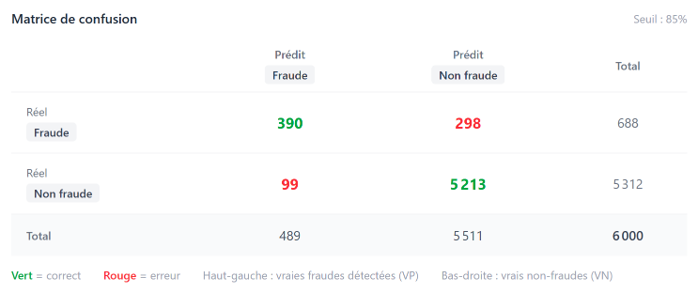
\includegraphics[width=0.9\textwidth]{images/chapitre5/boost/matrice_confusion_85_boost.png}
    \caption{Matrice de confusion du modèle Gradient Boosting pour un seuil de 85~\%}
    \label{fig:matrice-85-boost}
\end{figure}

\underline{Cette matrice permet de calculer} :

\begin{itemize}
    \item Le taux de non-fraudes bien classées (prédit non-fraudes / réel non-fraude total) : $5\,213 / 5\,312 = 98{,}14~\%$ ;
    \item Le taux de fraude détectées (prédit fraude / réel fraude) : $390 / 688 = 56{,}69~\%$.
    \item Le taux de sinistres signalés frauduleux : prédit fraude / total = $489 / 6\,000 = 8{,}15~\%$.
\end{itemize}

Néanmoins, la méthode graphique de détermination du seuil n'est pas toujours la meilleure et une optimisation du seuil afin d'obtenir la meilleure qualité de modèle est proposée dans le passage suivant.

% --------------------------------------------------------------
\subsection{Qualité du modèle obtenu}
% --------------------------------------------------------------

Le recours à une méthode ensembliste comme le Gradient \textit{Boosting} marque une rupture en termes de performance. Le modèle parvient à capturer des relations complexes et non linéaires, ce qui se traduit par une courbe de risque nettement plus régulière et globalement monotone.

La concentration des fraudes dans les tranches de probabilité élevées est particulièrement marquée, avec des taux proches de 100~\% sur les segments les plus extrêmes (sur données d'apprentissage).

Les indicateurs présentés dans cette partie sont l'application pratique des critères de qualité des modèles mis en place présentés en section~\ref{sec:criteres-evaluation}.

Pour commencer, on cherche le seuil optimal à partir duquel on peut considérer que les sinistres sont frauduleux à l'aide de l'indicateur de Youden (présenté en section~\ref{sec:qualite-modele}). Pour le modèle utilisant de Gradient \textit{Boosting}, le seuil optimal est de 50~\%.

\begin{figure}[H]
    \centering
    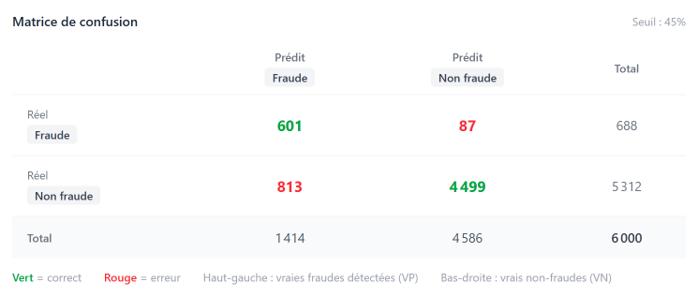
\includegraphics[width=0.9\textwidth]{images/chapitre5/boost/matrice_confusion_optimal_45_boost.png}
    \caption{Matrice de confusion du modèle Gradient Boosting avec un seuil de 45~\%}
    \label{fig:matrice-optimal-boost}
\end{figure}

\underline{Cette matrice permet de calculer} :

\begin{itemize}[label = $\bullet$]
    \item Le taux de non-fraudes bien classées (prédit non-fraudes / réel non-fraude total) : $4\,499 / 5\,312 = 84{,}69~\%$ ;
    \item Le taux de fraude détectées (prédit fraude / réel fraude) : $601 / 688 = 87{,}35~\%$ ;
    \item Le taux de sinistres signalés frauduleux : prédit fraude / total = $1\,414 / 6\,000 = 23{,}57~\%$.
\end{itemize}

L'efficacité opérationnelle de l'outil se mesure aussi à sa capacité à concentrer la fraude dans un volume restreint de dossiers à investiguer. Au seuil retenu, le modèle signale 23,57~\% des sinistres, parmi lesquels 87,35~\% sont réellement frauduleux, soit une densité de fraude environ 7,6 fois supérieure à celle d'un contrôle aléatoire. L'outil permet ainsi aux gestionnaires de concentrer leurs efforts sur un sous-ensemble à forte valeur, plutôt que de traiter l'ensemble du portefeuille.
%calcul du 7,6 : 87,35 / 11,5 = 7,6

\underline{À présent, observons les autres indicateurs de qualité du modèle} :

\begin{figure}[H]
    \centering
    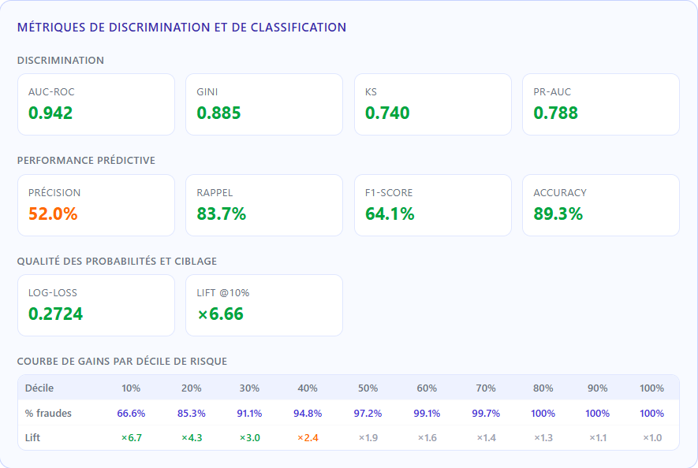
\includegraphics[width=0.9\textwidth]{images/chapitre5/boost/synthese_metrique_boost.png}
    \caption{Synthèse des métriques de discrimination et classification du modèle Gradient Boosting au seuil 45~\%}
    \label{fig:synthese-boost}
\end{figure}

\begin{figure}[H]
    \centering
    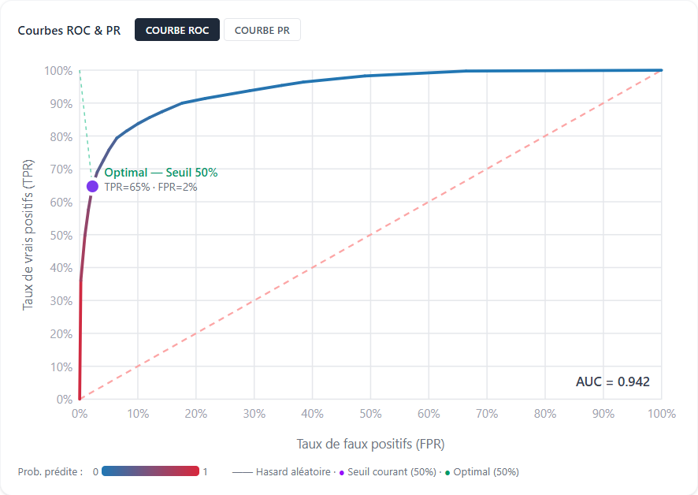
\includegraphics[width=0.9\textwidth]{images/chapitre5/boost/courbe_roc_auc_boost.png}
    \caption{Courbe ROC et AUC pour le modèle Gradient Boosting}
    \label{fig:roc-boost}
\end{figure}

En retenant le seuil optimal de 45~\%, les indicateurs obtenus s'interprètent de la façon suivante :

\begin{itemize}[label = $\bullet$]
    \item \textbf{AUC-ROC (0,933)} : excellente capacité de discrimination, très au-dessus du seuil de 0,8 considéré comme bon ; le modèle sépare efficacement fraudeurs et non-fraudeurs.
    \item \textbf{Gini (0,867)} : cohérent avec l'AUC, ce niveau traduit un pouvoir discriminant élevé, largement supérieur aux standards habituels en assurance.
    \item \textbf{KS (0,724)} : bien au-delà du seuil de 0,5, il confirme une nette séparation entre les distributions de scores des deux populations.
    \item \textbf{Précision (42,5~\%)} : parmi les dossiers signalés comme frauduleux, un peu moins d'un sur deux l'est réellement. Valeur modérée, mais attendue à ce seuil abaissé et acceptable au vu de l'objectif de détection.
    \item \textbf{Rappel (87,4~\%)} : le modèle détecte plus de quatre fraudes sur cinq, ce qui est le point fort de ce seuil et l'objectif prioritaire en détection de fraude.
    \item \textbf{F1-score (57,2~\%)} : bon compromis entre précision et rappel.
    \item \textbf{Accuracy (85,0~\%)} : taux de bonnes classifications élevé.
    \item \textbf{Log-loss (0,3131)} : valeur faible, signe d'une bonne calibration des probabilités prédites.
\end{itemize}   
 
Enfin, concernant les indicateurs de robustesse et stabilité du modèle, les résultats suivants sont obtenus :

\begin{itemize}[label = $\bullet$]
    \item {Backtesting (écart AUC train/test de 0,016)} : écart très faible entre apprentissage et test, signalant une excellente capacité de généralisation et l'absence de surapprentissage.
    \item \textbf{PSI (0,0023)} : très inférieur à 0,1, il atteste d'une bonne stabilité de la distribution des scores.
\end{itemize}


\begin{figure}[H]
    \centering
    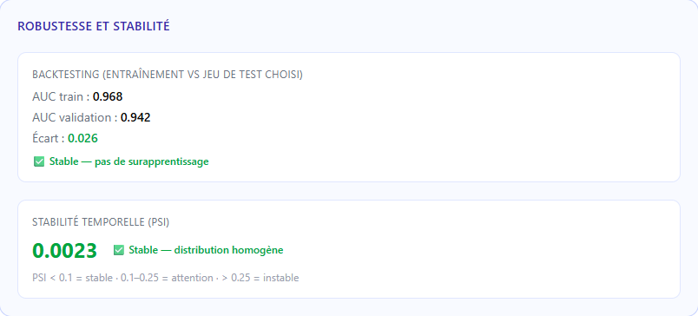
\includegraphics[width=0.9\textwidth]{images/chapitre5/boost/robustesse_boost.png}
    \caption{Indicateurs de robustesse et stabilité du modèle Gradient Boosting}
    \label{fig:robustesse-boost}
\end{figure}

% --------------------------------------------------------------
\subsection{Limites et précautions d'interprétation}
% --------------------------------------------------------------

Le Gradient \textit{Boosting} constitue le modèle le plus performant de cette étude, grâce à sa capacité à combiner un grand nombre d'arbres faibles corrigeant successivement leurs erreurs. Cette puissance s'accompagne toutefois de plusieurs limites qu'il convient de considérer dans une utilisation opérationnelle.

En premier lieu, le Gradient \textit{Boosting} est un modèle nettement moins interprétable que les précédents. Là où un arbre unique ou un \textit{scoring à point} offrent une lecture directe des règles de décision, la combinaison de deux cents arbres rend la logique globale difficile à retracer.

L'interprétation ne peut plus se faire directement sur la structure du modèle et nécessite le recours à des méthodes d'explicabilité complémentaires (importance des variables, valeurs de Shapley), qui restent des approximations et demandent une expertise spécifique.

Par ailleurs, le modèle est particulièrement sensible au réglage de ses hyperparamètres. Le nombre d'arbres, la profondeur, le taux d'apprentissage ou le sous-échantillonnage influencent fortement la performance et la robustesse : un paramétrage mal maîtrisé peut conduire à un surapprentissage, le modèle s'ajustant trop finement aux données d'entraînement au détriment de sa capacité de généralisation. Un encadrement méthodologique rigoureux, via une validation appropriée, est donc indispensable.

En outre, comme tout modèle supervisé, le Gradient \textit{Boosting} reste dépendant de la qualité et de la représentativité des données historiques. Il peut amplifier certains biais présents dans les données (biais de détection ou d'investigation) et reproduire des schémas passés qui ne reflètent pas nécessairement les fraudes futures.

Enfin, la calibration des probabilités mérite attention : les scores produits ne sont pas toujours directement interprétables comme des probabilités exactes, ce qui justifie une étape de calibration et un choix réfléchi du seuil de décision.

Ainsi, le Gradient \textit{Boosting} offre les meilleures performances prédictives de l'étude, mais au prix d'une moindre interprétabilité et d'une plus grande complexité de mise en œuvre, qui imposent un cadre de validation et de suivi rigoureux.

% ==============================================================
\section{Comparaison des modèles}
% ==============================================================

Une fois les trois modèles présentés, le passage ci-dessous a pour objet de faire une synthèse et comparaison des résultats obtenus pour orienter le choix du modèle finalement retenu parmi les trois modèles testés par l'Agent IA.

Ci-dessous, un tableau récapitulatif des différents indicateurs de qualité selon le modèle testé.

\begin{table}[H]
    \centering
    \renewcommand{\arraystretch}{1.4}
    \begin{tabularx}{\textwidth}{|>{\raggedright\arraybackslash}p{3.5cm}|>{\centering\arraybackslash}X|>{\centering\arraybackslash}X|>{\centering\arraybackslash}X|}
        \hline
        \rowcolor{accenture}
        \textcolor{white}{\textbf{Indicateur}} & \textcolor{white}{\textbf{Scoring en point}} & \textcolor{white}{\textbf{Arbre de décision}} & \textcolor{white}{\textbf{Gradient Boosting}} \\
        \hline
        \textbf{AUC-ROC} & 0,917 & 0,845 & \textbf{0,933} \\
        \hline
        \textbf{Gini} & 0,835 & 0,690 & \textbf{0,867} \\
        \hline
        \textbf{KS} & 0,666 & 0,564 & \textbf{0,724} \\
        \hline
        \textbf{Lift @10~\%} & --- & $\times$4,83 & \textbf{$\times$6,37} \\
        \hline
        \textbf{PSI} & 0,0026 & 0,0026 & \textbf{0,0023} \\
        \hline
        \textbf{Écart Backtesting} & \textbf{0,003} & 0,039 & 0,016 \\
        \hline
    \end{tabularx}
    \caption{Synthèse des résultats des indicateurs de qualité des différents modèles}
    \label{tab:synthese-modeles}
\end{table}

\subsubsection*{Stabilité et robustesse des modèles}

Les trois modèles présentent une stabilité temporelle remarquable, avec des valeurs de PSI très inférieures au seuil d'alerte de 0,10 (0,003 pour le \textit{scoring en points}, 0,0026 pour l'arbre de décision et 0,0023 pour le gradient boosting). Ces valeurs attestent d'une distribution homogène des scores entre les échantillons d'entraînement et de validation, et confirment que les modèles ne sont pas sensibles à des dérives temporelles sur la période considérée. Par ailleurs, le \textit{backtesting} en split 80/20 révèle une bonne capacité de généralisation : les écarts entre AUC d'entraînement et AUC de validation restent contenus (0,009 pour le \textit{scoring} en points, 0,039 pour l'arbre de décision et 0,016 pour le Gradient \textit{Boosting}). Le \textit{scoring en points} affiche l'écart le plus faible, cohérent avec sa simplicité, tandis que le modèle basé sur les arbres de décision présente l'écart le plus marqué, traduisant sa tendance connue au surapprentissage ; celui-ci reste toutefois modéré et n'entame pas significativement la robustesse du modèle.

\subsubsection*{Analyse du compromis précision / rappel et choix du seuil de décision}

Le Gradient \textit{Boosting} s'impose comme le modèle retenu à retenir, car il offre le meilleur pouvoir discriminant parmi les trois approches testées : une AUC de 0\,942, un indice de Gini de 0\,885 et un lift de $\times$6,66 au premier décile. Il devance nettement le modèle basé sur un arbre de décision (AUC de 0\,838, indice de Gini de 0\,676, lift de $\times$4,61) et, plus légèrement, le modèle basé sur un \textit{scoring} en points (AUC de 0\,923, indice de Gini de 0\,846). Sa capacité à concentrer la fraude dans les premiers déciles en fait l'outil le plus efficace pour prioriser les dossiers à investiguer, ce qui correspond précisément à l'objectif opérationnel poursuivi.

Ce choix ne disqualifie pas pour autant le modèle basé sur un \textbf{\textit{scoring} en points, qui demeure un modèle remarquablement performant au regard de sa simplicité}. Avec une AUC de 0,923 et un indice de Gini de 0,846, il se situe très près du Gradient Boosting et loin devant l'arbre de décision, tout en conservant une transparence et une interprétabilité que les méthodes d'ensemble ne permettent pas. Il constitue donc une alternative pleinement crédible lorsque l'explicabilité prime sur le dernier point de performance, par exemple pour une présentation aux gestionnaires ou dans un contexte réglementaire exigeant. Le choix entre ces deux modèles relève ainsi d'un arbitrage entre performance pure (Gradient \textit{Boosting}) et interprétabilité (\text{scoring} en points), l'arbre de décision étant quant à lui écarté, dominé sur l'ensemble des critères.

Enfin, quel que soit le modèle retenu, la lecture des performances appelle une nuance commune. Le compromis entre précision et rappel est la conséquence directe du fort déséquilibre des classes dans les données de sinistres. D'un point de vue actuariel, ce ratio doit être piloté explicitement : modifier le seuil de décision permet d'ajuster le rappel au prix d'un volume plus ou moins élevé de dossiers à investiguer.

Enfin, quel que soit le modèle retenu, la lecture des performances appelle une nuance commune, liée à la tension inhérente entre précision et rappel. Ces deux indicateurs évoluent en sens inverse selon le seuil de décision : abaisser le seuil permet de détecter davantage de fraudes (rappel plus élevé), mais au prix d'un plus grand nombre de dossiers sains signalés à tort (précision plus faible), et inversement.. D'un point de vue actuariel, ce ratio doit être piloté explicitement : modifier le seuil de décision permet d'ajuster le rappel au prix d'un volume plus ou moins élevé de dossiers à investiguer. Le choix optimal de ce curseur dépend du coût asymétrique des deux types d'erreurs : un faux négatif (fraude non détectée) engendre une perte indemnisée à tort, tandis qu'un faux positif (investigation inutile) représente un coût opérationnel pour la cellule fraude. C'est précisément pour cette raison que l'outil développé laisse à l'utilisateur le soin de manipuler dynamiquement le curseur des seuils de détection, afin d'adapter le dispositif au contexte et à l'appétence au risque de chaque assureur.

\subsubsection*{Configuration finale du modèle}

La dernière étape de l'Agent IA de création du modèle d'aide à la détection de fraude consiste à l'enregistrement du modèle choisi.

Pour ce faire, l'utilisateur doit confirmer le modèle retenu ainsi que le seuil optimal.

Un seuil d'investigation fixé par défaut à $\pm$10~\%\footnote{Ces seuils d'investigation peuvent être modifiés par l'utilisateur s'il le souhaite.} du seuil optimal sera retenu, ainsi, si l'on considère par exemple un seuil optimal de 45~\%, trois zones d'investigations seront mises en place :

\begin{itemize}[label = $\bullet$]
    \item \textcolor{vert}{Probabilité de fraude $<$ 35~\% : pas d'investigation}
    \item \textcolor{orange}{Probabilité de fraude entre 35~\% et 55~\% : investigation légère}
    \item \textcolor{rouge}{Probabilité de fraude supérieure à 55~\% : investigation à lancer}
\end{itemize}

Dans notre cas, on choisit le modèle Gradient \textit{Boosting} avec les seuils 35~\% et 55~\% .

\begin{figure}[H]
    \centering
    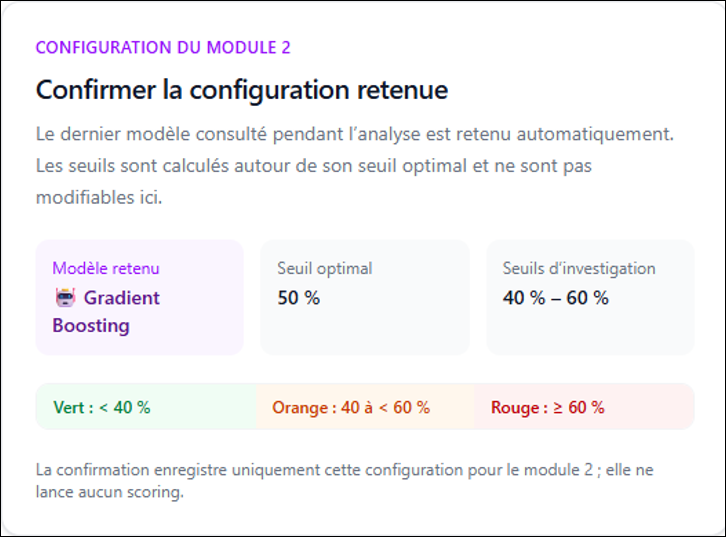
\includegraphics[width=0.9\textwidth]{images/chapitre5/configuration.png}
    \caption{Configuration finale du modèle et des seuils d'investigation}
    \label{fig:configuration}
\end{figure}

Une fois cette dernière étape réalisée, l'outil mis à disposition du service de détection des fraudes est configuré avec ce modèle et ces seuils d'investigation.

Ces derniers ne sont pas modifiables dans le second outil. Seul le premier Agent IA doit être relancé pour modifier le modèle sous-jacent de modélisation de la probabilité de fraude.